% Options for packages loaded elsewhere
\PassOptionsToPackage{unicode}{hyperref}
\PassOptionsToPackage{hyphens}{url}
%
\documentclass[
]{article}
\usepackage{amsmath,amssymb}
\usepackage{iftex}
\ifPDFTeX
  \usepackage[T1]{fontenc}
  \usepackage[utf8]{inputenc}
  \usepackage{textcomp} % provide euro and other symbols
\else % if luatex or xetex
  \usepackage{unicode-math} % this also loads fontspec
  \defaultfontfeatures{Scale=MatchLowercase}
  \defaultfontfeatures[\rmfamily]{Ligatures=TeX,Scale=1}
\fi
\usepackage{lmodern}
\ifPDFTeX\else
  % xetex/luatex font selection
\fi
% Use upquote if available, for straight quotes in verbatim environments
\IfFileExists{upquote.sty}{\usepackage{upquote}}{}
\IfFileExists{microtype.sty}{% use microtype if available
  \usepackage[]{microtype}
  \UseMicrotypeSet[protrusion]{basicmath} % disable protrusion for tt fonts
}{}
\makeatletter
\@ifundefined{KOMAClassName}{% if non-KOMA class
  \IfFileExists{parskip.sty}{%
    \usepackage{parskip}
  }{% else
    \setlength{\parindent}{0pt}
    \setlength{\parskip}{6pt plus 2pt minus 1pt}}
}{% if KOMA class
  \KOMAoptions{parskip=half}}
\makeatother
\usepackage{xcolor}
\usepackage[margin=1in]{geometry}
\usepackage{color}
\usepackage{fancyvrb}
\newcommand{\VerbBar}{|}
\newcommand{\VERB}{\Verb[commandchars=\\\{\}]}
\DefineVerbatimEnvironment{Highlighting}{Verbatim}{commandchars=\\\{\}}
% Add ',fontsize=\small' for more characters per line
\usepackage{framed}
\definecolor{shadecolor}{RGB}{248,248,248}
\newenvironment{Shaded}{\begin{snugshade}}{\end{snugshade}}
\newcommand{\AlertTok}[1]{\textcolor[rgb]{0.94,0.16,0.16}{#1}}
\newcommand{\AnnotationTok}[1]{\textcolor[rgb]{0.56,0.35,0.01}{\textbf{\textit{#1}}}}
\newcommand{\AttributeTok}[1]{\textcolor[rgb]{0.13,0.29,0.53}{#1}}
\newcommand{\BaseNTok}[1]{\textcolor[rgb]{0.00,0.00,0.81}{#1}}
\newcommand{\BuiltInTok}[1]{#1}
\newcommand{\CharTok}[1]{\textcolor[rgb]{0.31,0.60,0.02}{#1}}
\newcommand{\CommentTok}[1]{\textcolor[rgb]{0.56,0.35,0.01}{\textit{#1}}}
\newcommand{\CommentVarTok}[1]{\textcolor[rgb]{0.56,0.35,0.01}{\textbf{\textit{#1}}}}
\newcommand{\ConstantTok}[1]{\textcolor[rgb]{0.56,0.35,0.01}{#1}}
\newcommand{\ControlFlowTok}[1]{\textcolor[rgb]{0.13,0.29,0.53}{\textbf{#1}}}
\newcommand{\DataTypeTok}[1]{\textcolor[rgb]{0.13,0.29,0.53}{#1}}
\newcommand{\DecValTok}[1]{\textcolor[rgb]{0.00,0.00,0.81}{#1}}
\newcommand{\DocumentationTok}[1]{\textcolor[rgb]{0.56,0.35,0.01}{\textbf{\textit{#1}}}}
\newcommand{\ErrorTok}[1]{\textcolor[rgb]{0.64,0.00,0.00}{\textbf{#1}}}
\newcommand{\ExtensionTok}[1]{#1}
\newcommand{\FloatTok}[1]{\textcolor[rgb]{0.00,0.00,0.81}{#1}}
\newcommand{\FunctionTok}[1]{\textcolor[rgb]{0.13,0.29,0.53}{\textbf{#1}}}
\newcommand{\ImportTok}[1]{#1}
\newcommand{\InformationTok}[1]{\textcolor[rgb]{0.56,0.35,0.01}{\textbf{\textit{#1}}}}
\newcommand{\KeywordTok}[1]{\textcolor[rgb]{0.13,0.29,0.53}{\textbf{#1}}}
\newcommand{\NormalTok}[1]{#1}
\newcommand{\OperatorTok}[1]{\textcolor[rgb]{0.81,0.36,0.00}{\textbf{#1}}}
\newcommand{\OtherTok}[1]{\textcolor[rgb]{0.56,0.35,0.01}{#1}}
\newcommand{\PreprocessorTok}[1]{\textcolor[rgb]{0.56,0.35,0.01}{\textit{#1}}}
\newcommand{\RegionMarkerTok}[1]{#1}
\newcommand{\SpecialCharTok}[1]{\textcolor[rgb]{0.81,0.36,0.00}{\textbf{#1}}}
\newcommand{\SpecialStringTok}[1]{\textcolor[rgb]{0.31,0.60,0.02}{#1}}
\newcommand{\StringTok}[1]{\textcolor[rgb]{0.31,0.60,0.02}{#1}}
\newcommand{\VariableTok}[1]{\textcolor[rgb]{0.00,0.00,0.00}{#1}}
\newcommand{\VerbatimStringTok}[1]{\textcolor[rgb]{0.31,0.60,0.02}{#1}}
\newcommand{\WarningTok}[1]{\textcolor[rgb]{0.56,0.35,0.01}{\textbf{\textit{#1}}}}
\usepackage{graphicx}
\makeatletter
\newsavebox\pandoc@box
\newcommand*\pandocbounded[1]{% scales image to fit in text height/width
  \sbox\pandoc@box{#1}%
  \Gscale@div\@tempa{\textheight}{\dimexpr\ht\pandoc@box+\dp\pandoc@box\relax}%
  \Gscale@div\@tempb{\linewidth}{\wd\pandoc@box}%
  \ifdim\@tempb\p@<\@tempa\p@\let\@tempa\@tempb\fi% select the smaller of both
  \ifdim\@tempa\p@<\p@\scalebox{\@tempa}{\usebox\pandoc@box}%
  \else\usebox{\pandoc@box}%
  \fi%
}
% Set default figure placement to htbp
\def\fps@figure{htbp}
\makeatother
\setlength{\emergencystretch}{3em} % prevent overfull lines
\providecommand{\tightlist}{%
  \setlength{\itemsep}{0pt}\setlength{\parskip}{0pt}}
\setcounter{secnumdepth}{-\maxdimen} % remove section numbering
\usepackage{bookmark}
\IfFileExists{xurl.sty}{\usepackage{xurl}}{} % add URL line breaks if available
\urlstyle{same}
\hypersetup{
  pdftitle={glmCH1},
  hidelinks,
  pdfcreator={LaTeX via pandoc}}

\title{glmCH1}
\author{}
\date{\vspace{-2.5em}}

\begin{document}
\maketitle

\section{Load and clean data}\label{load-and-clean-data}

\begin{Shaded}
\begin{Highlighting}[]
\CommentTok{\#load packages}
\FunctionTok{library}\NormalTok{(tidyverse)}
\end{Highlighting}
\end{Shaded}

\begin{verbatim}
## -- Attaching core tidyverse packages ------------------------ tidyverse 2.0.0 --
## v dplyr     1.1.4     v readr     2.1.5
## v forcats   1.0.0     v stringr   1.5.1
## v ggplot2   3.5.2     v tibble    3.3.0
## v lubridate 1.9.4     v tidyr     1.3.1
## v purrr     1.0.4     
## -- Conflicts ------------------------------------------ tidyverse_conflicts() --
## x dplyr::filter() masks stats::filter()
## x dplyr::lag()    masks stats::lag()
## i Use the conflicted package (<http://conflicted.r-lib.org/>) to force all conflicts to become errors
\end{verbatim}

\begin{Shaded}
\begin{Highlighting}[]
\FunctionTok{library}\NormalTok{(ggplot2)}
\FunctionTok{library}\NormalTok{(DHARMa)}
\end{Highlighting}
\end{Shaded}

\begin{verbatim}
## This is DHARMa 0.4.7. For overview type '?DHARMa'. For recent changes, type news(package = 'DHARMa')
\end{verbatim}

\begin{Shaded}
\begin{Highlighting}[]
\FunctionTok{library}\NormalTok{(glmmTMB)}

\CommentTok{\#read in data}
\NormalTok{data }\OtherTok{\textless{}{-}} \FunctionTok{read.csv}\NormalTok{(}\StringTok{"06\_cleandata/combined\_plot\_data.csv"}\NormalTok{)}

\CommentTok{\#check that variables are in appropriate format}
\FunctionTok{str}\NormalTok{(data)}
\end{Highlighting}
\end{Shaded}

\begin{verbatim}
## 'data.frame':    210 obs. of  34 variables:
##  $ site_id                 : chr  "bates_57b" "bates_57b" "bates_57b" "bates_57b" ...
##  $ round                   : chr  "2024_r1" "2024_r1" "2024_r1" "2024_r2" ...
##  $ plot_id                 : chr  "p1" "p2" "d" "p1" ...
##  $ bee_date                : chr  "2024-04-15" "2024-04-15" "2024-04-15" "2024-06-06" ...
##  $ julian.date             : int  106 106 106 158 158 158 173 173 173 101 ...
##  $ bee_season_type         : chr  "nestsearching" "nestsearching" "nestsearching" "worker" ...
##  $ area                    : chr  "delta_1" "delta_1" "delta_1" "delta_1" ...
##  $ cover_type              : chr  "grass" "grass" "grass" "grass" ...
##  $ bare_perc               : num  2 1.42 0 11.92 20.5 ...
##  $ grass_perc              : num  46.8 52.2 90.4 52.7 56.8 ...
##  $ forb_perc               : num  9.33 7.92 8 16.75 8.12 ...
##  $ grass_forb_perc         : num  56.2 60.2 98.4 69.4 64.9 ...
##  $ grass_h                 : num  17.9 19.5 28.8 25.3 25.7 ...
##  $ forb_h                  : num  9.83 7.42 9.58 26.17 17.42 ...
##  $ floral_perc             : num  0.375 1.0417 0.125 0.0417 0 ...
##  $ bombus_floral_perc      : num  0.375 1.0417 0.0833 0.0417 0 ...
##  $ grass_forb_floral_perc  : num  56.5 61.2 98.5 69.5 64.9 ...
##  $ flood_perc              : num  0 0 0 0 0 0 0 0 0 0 ...
##  $ dry_root_perc           : num  25.42 37.17 7.08 16.25 5.42 ...
##  $ bryo_perc               : num  0 0 0 0 0 0 0 0 0 0 ...
##  $ bare_flood_dry_bryo_perc: num  27.42 38.58 7.08 28.17 25.92 ...
##  $ bare_dry_bryo_perc      : num  27.42 38.58 7.08 28.17 25.92 ...
##  $ floral_richness         : int  1 1 3 2 3 14 2 2 12 2 ...
##  $ bombus_floral_richness  : int  1 1 2 2 3 11 2 2 10 2 ...
##  $ floral_abun             : num  3 3 3.32 2.01 2.01 ...
##  $ bombus_floral_abun      : num  3 3 3.04 2.01 2.01 ...
##  $ nest_searching_queens   : int  3 0 4 2 0 0 0 0 0 0 ...
##  $ workers                 : int  1 0 0 0 1 2 0 0 0 0 ...
##  $ forage_vaco             : int  1 2 0 2 4 0 0 0 0 3 ...
##  $ num_burrows             : int  41 120 93 41 120 93 41 120 93 41 ...
##  $ num_inactive_burrows    : int  10 64 0 10 64 0 10 64 0 10 ...
##  $ num_active_dm           : int  5 6 0 5 6 0 5 6 0 5 ...
##  $ num_dm_size             : int  3 3 0 3 3 0 3 3 0 3 ...
##  $ num_inactive_dm         : int  1 2 0 1 2 0 1 2 0 1 ...
\end{verbatim}

\begin{Shaded}
\begin{Highlighting}[]
\CommentTok{\#change character columns to factors}
\NormalTok{surveys }\OtherTok{\textless{}{-}}\NormalTok{ data }\SpecialCharTok{\%\textgreater{}\%}
   \FunctionTok{mutate}\NormalTok{(}
     \AttributeTok{site\_id =} \FunctionTok{as.factor}\NormalTok{(site\_id),}
     \AttributeTok{round =} \FunctionTok{as.factor}\NormalTok{(round),}
     \AttributeTok{plot\_id =} \FunctionTok{as.factor}\NormalTok{(plot\_id),}
     \AttributeTok{bee\_date =} \FunctionTok{as.Date}\NormalTok{(bee\_date),}
     \AttributeTok{bee\_season\_type =} \FunctionTok{as.factor}\NormalTok{(bee\_season\_type),}
     \AttributeTok{area =} \FunctionTok{as.factor}\NormalTok{(area))}
\end{Highlighting}
\end{Shaded}

Scale continuous predictors

\begin{Shaded}
\begin{Highlighting}[]
\NormalTok{surveys}\SpecialCharTok{$}\NormalTok{julian.date\_scaled }\OtherTok{\textless{}{-}} \FunctionTok{as.numeric}\NormalTok{(}\FunctionTok{scale}\NormalTok{(surveys}\SpecialCharTok{$}\NormalTok{julian.date))}
\NormalTok{surveys}\SpecialCharTok{$}\NormalTok{bare\_perc\_scaled }\OtherTok{\textless{}{-}} \FunctionTok{as.numeric}\NormalTok{(}\FunctionTok{scale}\NormalTok{(surveys}\SpecialCharTok{$}\NormalTok{bare\_perc))}
\NormalTok{surveys}\SpecialCharTok{$}\NormalTok{grass\_perc\_scaled }\OtherTok{\textless{}{-}} \FunctionTok{as.numeric}\NormalTok{(}\FunctionTok{scale}\NormalTok{(surveys}\SpecialCharTok{$}\NormalTok{grass\_perc))}
\NormalTok{surveys}\SpecialCharTok{$}\NormalTok{forb\_perc\_scaled }\OtherTok{\textless{}{-}} \FunctionTok{as.numeric}\NormalTok{(}\FunctionTok{scale}\NormalTok{(surveys}\SpecialCharTok{$}\NormalTok{forb\_perc))}
\NormalTok{surveys}\SpecialCharTok{$}\NormalTok{grass\_forb\_perc\_scaled }\OtherTok{\textless{}{-}} \FunctionTok{as.numeric}\NormalTok{(}\FunctionTok{scale}\NormalTok{(surveys}\SpecialCharTok{$}\NormalTok{grass\_forb\_perc))}
\NormalTok{surveys}\SpecialCharTok{$}\NormalTok{grass\_h\_scaled }\OtherTok{\textless{}{-}} \FunctionTok{as.numeric}\NormalTok{(}\FunctionTok{scale}\NormalTok{(surveys}\SpecialCharTok{$}\NormalTok{grass\_h))}
\NormalTok{surveys}\SpecialCharTok{$}\NormalTok{forb\_h\_scaled }\OtherTok{\textless{}{-}} \FunctionTok{as.numeric}\NormalTok{(}\FunctionTok{scale}\NormalTok{(surveys}\SpecialCharTok{$}\NormalTok{forb\_h))}
\NormalTok{surveys}\SpecialCharTok{$}\NormalTok{floral\_perc\_scaled }\OtherTok{\textless{}{-}} \FunctionTok{as.numeric}\NormalTok{(}\FunctionTok{scale}\NormalTok{(surveys}\SpecialCharTok{$}\NormalTok{floral\_perc))}
\NormalTok{surveys}\SpecialCharTok{$}\NormalTok{grass\_forb\_floral\_perc\_scaled }\OtherTok{\textless{}{-}} \FunctionTok{as.numeric}\NormalTok{(}\FunctionTok{scale}\NormalTok{(surveys}\SpecialCharTok{$}\NormalTok{grass\_forb\_floral\_perc))}
\NormalTok{surveys}\SpecialCharTok{$}\NormalTok{bombus\_floral\_perc\_scaled }\OtherTok{\textless{}{-}} \FunctionTok{as.numeric}\NormalTok{(}\FunctionTok{scale}\NormalTok{(surveys}\SpecialCharTok{$}\NormalTok{bombus\_floral\_perc))}
\NormalTok{surveys}\SpecialCharTok{$}\NormalTok{flood\_perc\_scaled }\OtherTok{\textless{}{-}} \FunctionTok{as.numeric}\NormalTok{(}\FunctionTok{scale}\NormalTok{(surveys}\SpecialCharTok{$}\NormalTok{flood\_perc))}
\NormalTok{surveys}\SpecialCharTok{$}\NormalTok{dry\_root\_perc\_scaled }\OtherTok{\textless{}{-}} \FunctionTok{as.numeric}\NormalTok{(}\FunctionTok{scale}\NormalTok{(surveys}\SpecialCharTok{$}\NormalTok{dry\_root\_perc))}
\NormalTok{surveys}\SpecialCharTok{$}\NormalTok{bryo\_perc\_scaled }\OtherTok{\textless{}{-}} \FunctionTok{as.numeric}\NormalTok{(}\FunctionTok{scale}\NormalTok{(surveys}\SpecialCharTok{$}\NormalTok{bryo\_perc))}
\NormalTok{surveys}\SpecialCharTok{$}\NormalTok{bare\_flood\_dry\_bryo\_perc\_scaled }\OtherTok{\textless{}{-}} \FunctionTok{as.numeric}\NormalTok{(}\FunctionTok{scale}\NormalTok{(surveys}\SpecialCharTok{$}\NormalTok{bare\_flood\_dry\_bryo\_perc))}
\NormalTok{surveys}\SpecialCharTok{$}\NormalTok{floral\_richness\_scaled }\OtherTok{\textless{}{-}} \FunctionTok{as.numeric}\NormalTok{(}\FunctionTok{scale}\NormalTok{(surveys}\SpecialCharTok{$}\NormalTok{floral\_richness))}
\NormalTok{surveys}\SpecialCharTok{$}\NormalTok{bombus\_floral\_richness\_scaled }\OtherTok{\textless{}{-}} \FunctionTok{as.numeric}\NormalTok{(}\FunctionTok{scale}\NormalTok{(surveys}\SpecialCharTok{$}\NormalTok{bombus\_floral\_richness))}
\NormalTok{surveys}\SpecialCharTok{$}\NormalTok{floral\_abun\_scaled }\OtherTok{\textless{}{-}} \FunctionTok{as.numeric}\NormalTok{(}\FunctionTok{scale}\NormalTok{(surveys}\SpecialCharTok{$}\NormalTok{floral\_abun))}
\NormalTok{surveys}\SpecialCharTok{$}\NormalTok{bombus\_floral\_abun\_scaled }\OtherTok{\textless{}{-}} \FunctionTok{as.numeric}\NormalTok{(}\FunctionTok{scale}\NormalTok{(surveys}\SpecialCharTok{$}\NormalTok{bombus\_floral\_abun))}
\NormalTok{surveys}\SpecialCharTok{$}\NormalTok{nest\_searching\_queens\_scaled }\OtherTok{\textless{}{-}} \FunctionTok{as.numeric}\NormalTok{(}\FunctionTok{scale}\NormalTok{(surveys}\SpecialCharTok{$}\NormalTok{nest\_searching\_queens))}
\NormalTok{surveys}\SpecialCharTok{$}\NormalTok{workers\_scaled }\OtherTok{\textless{}{-}} \FunctionTok{as.numeric}\NormalTok{(}\FunctionTok{scale}\NormalTok{(surveys}\SpecialCharTok{$}\NormalTok{workers))}
\NormalTok{surveys}\SpecialCharTok{$}\NormalTok{forage\_vaco\_scaled }\OtherTok{\textless{}{-}} \FunctionTok{as.numeric}\NormalTok{(}\FunctionTok{scale}\NormalTok{(surveys}\SpecialCharTok{$}\NormalTok{forage\_vaco))}
\NormalTok{surveys}\SpecialCharTok{$}\NormalTok{num\_burrows\_scaled }\OtherTok{\textless{}{-}} \FunctionTok{as.numeric}\NormalTok{(}\FunctionTok{scale}\NormalTok{(surveys}\SpecialCharTok{$}\NormalTok{num\_burrows))}
\NormalTok{surveys}\SpecialCharTok{$}\NormalTok{num\_inactive\_burrows\_scaled }\OtherTok{\textless{}{-}} \FunctionTok{as.numeric}\NormalTok{(}\FunctionTok{scale}\NormalTok{(surveys}\SpecialCharTok{$}\NormalTok{num\_inactive\_burrows))}
\NormalTok{surveys}\SpecialCharTok{$}\NormalTok{num\_active\_dm\_scaled }\OtherTok{\textless{}{-}} \FunctionTok{as.numeric}\NormalTok{(}\FunctionTok{scale}\NormalTok{(surveys}\SpecialCharTok{$}\NormalTok{num\_active\_dm))}
\NormalTok{surveys}\SpecialCharTok{$}\NormalTok{num\_dm\_size\_scaled }\OtherTok{\textless{}{-}} \FunctionTok{as.numeric}\NormalTok{(}\FunctionTok{scale}\NormalTok{(surveys}\SpecialCharTok{$}\NormalTok{num\_dm\_size))}
\NormalTok{surveys}\SpecialCharTok{$}\NormalTok{num\_inactive\_dm\_scaled }\OtherTok{\textless{}{-}} \FunctionTok{as.numeric}\NormalTok{(}\FunctionTok{scale}\NormalTok{(surveys}\SpecialCharTok{$}\NormalTok{num\_inactive\_dm))}
\end{Highlighting}
\end{Shaded}

Filter to only include field data

\begin{Shaded}
\begin{Highlighting}[]
\NormalTok{field\_data }\OtherTok{\textless{}{-}}\NormalTok{ surveys }\SpecialCharTok{\%\textgreater{}\%}
  \FunctionTok{filter}\NormalTok{(plot\_id }\SpecialCharTok{!=} \StringTok{"d"}\NormalTok{)}
\end{Highlighting}
\end{Shaded}

\section{GLM \#1: Number of nest-searching
queens}\label{glm-1-number-of-nest-searching-queens}

Plotting a zero-inflated poisson model

\begin{Shaded}
\begin{Highlighting}[]
\NormalTok{nsq\_lm\_zeroPois }\OtherTok{\textless{}{-}} \FunctionTok{glmmTMB}\NormalTok{(nest\_searching\_queens }\SpecialCharTok{\textasciitilde{}}\NormalTok{ grass\_forb\_perc\_scaled }\SpecialCharTok{+} 
\NormalTok{                    bombus\_floral\_abun\_scaled }\SpecialCharTok{+} 
\NormalTok{                    num\_burrows\_scaled }\SpecialCharTok{+} 
\NormalTok{                     num\_inactive\_burrows\_scaled }\SpecialCharTok{+} 
\NormalTok{                    bee\_season\_type, }
                  \AttributeTok{ziformula =} \SpecialCharTok{\textasciitilde{}}\DecValTok{1}\NormalTok{,  }\CommentTok{\# zero{-}inflation model}
                  \AttributeTok{family =}\NormalTok{ poisson, }\CommentTok{\#poisson}
                  \AttributeTok{data =}\NormalTok{ field\_data)}

\FunctionTok{summary}\NormalTok{(nsq\_lm\_zeroPois)}
\end{Highlighting}
\end{Shaded}

\begin{verbatim}
##  Family: poisson  ( log )
## Formula:          
## nest_searching_queens ~ grass_forb_perc_scaled + bombus_floral_abun_scaled +  
##     num_burrows_scaled + num_inactive_burrows_scaled + bee_season_type
## Zero inflation:                         ~1
## Data: field_data
## 
##       AIC       BIC    logLik -2*log(L)  df.resid 
##     151.3     171.9     -68.7     137.3       133 
## 
## 
## Conditional model:
##                             Estimate Std. Error z value Pr(>|z|)    
## (Intercept)                   0.2772     0.4464   0.621  0.53462    
## grass_forb_perc_scaled        0.2930     0.2493   1.175  0.23980    
## bombus_floral_abun_scaled     0.2277     0.2092   1.088  0.27652    
## num_burrows_scaled            2.3470     1.1074   2.119  0.03405 *  
## num_inactive_burrows_scaled  -1.9770     0.9995  -1.978  0.04793 *  
## bee_season_typeworker        -2.2642     0.6247  -3.624  0.00029 ***
## ---
## Signif. codes:  0 '***' 0.001 '**' 0.01 '*' 0.05 '.' 0.1 ' ' 1
## 
## Zero-inflation model:
##             Estimate Std. Error z value Pr(>|z|)
## (Intercept)  -0.5993     0.8062  -0.743    0.457
\end{verbatim}

Diagnostics

\begin{Shaded}
\begin{Highlighting}[]
\CommentTok{\#simulate residuals}

\NormalTok{residuals\_nsq\_zeroPois }\OtherTok{\textless{}{-}} \FunctionTok{simulateResiduals}\NormalTok{(}\AttributeTok{fittedModel =}\NormalTok{ nsq\_lm\_zeroPois, }\AttributeTok{plot =} \ConstantTok{TRUE}\NormalTok{)}
\end{Highlighting}
\end{Shaded}

\pandocbounded{
\includegraphics[keepaspectratio]{glmCH1_files/figure-latex/unnamed-chunk-5-1.pdf}}

\begin{Shaded}
\begin{Highlighting}[]
\DocumentationTok{\#\#no evidence of overdispersion or significant outliers}
\end{Highlighting}
\end{Shaded}

Plotting a binary model to predict if \#NSQ \textgreater{} 0

\begin{Shaded}
\begin{Highlighting}[]
\CommentTok{\#create binary variable for nsq presence}
\NormalTok{field\_data}\SpecialCharTok{$}\NormalTok{nsq\_binary }\OtherTok{\textless{}{-}} \FunctionTok{ifelse}\NormalTok{(field\_data}\SpecialCharTok{$}\NormalTok{nest\_searching\_queens }\SpecialCharTok{\textgreater{}} \DecValTok{0}\NormalTok{, }\DecValTok{1}\NormalTok{, }\DecValTok{0}\NormalTok{)}

\NormalTok{nsq\_lm\_binary }\OtherTok{\textless{}{-}} \FunctionTok{glmmTMB}\NormalTok{(nsq\_binary }\SpecialCharTok{\textasciitilde{}}\NormalTok{ grass\_forb\_perc\_scaled }\SpecialCharTok{+} 
\NormalTok{                    bombus\_floral\_abun\_scaled }\SpecialCharTok{+} 
\NormalTok{                    num\_burrows\_scaled }\SpecialCharTok{+} 
\NormalTok{                    num\_inactive\_burrows\_scaled }\SpecialCharTok{+} 
\NormalTok{                    bee\_season\_type, }
                  \AttributeTok{family =}\NormalTok{ binomial, }
                  \AttributeTok{data =}\NormalTok{ field\_data)}

\FunctionTok{summary}\NormalTok{(nsq\_lm\_binary)}
\end{Highlighting}
\end{Shaded}

\begin{verbatim}
##  Family: binomial  ( logit )
## Formula:          
## nsq_binary ~ grass_forb_perc_scaled + bombus_floral_abun_scaled +  
##     num_burrows_scaled + num_inactive_burrows_scaled + bee_season_type
## Data: field_data
## 
##       AIC       BIC    logLik -2*log(L)  df.resid 
##      97.8     115.4     -42.9      85.8       134 
## 
## 
## Conditional model:
##                             Estimate Std. Error z value Pr(>|z|)    
## (Intercept)                  -0.3569     0.6149  -0.580 0.561590    
## grass_forb_perc_scaled        1.0014     0.3596   2.785 0.005357 ** 
## bombus_floral_abun_scaled     0.4924     0.2880   1.710 0.087303 .  
## num_burrows_scaled            1.3950     1.7315   0.806 0.420430    
## num_inactive_burrows_scaled  -1.6596     1.4770  -1.124 0.261167    
## bee_season_typeworker        -2.6963     0.7890  -3.417 0.000633 ***
## ---
## Signif. codes:  0 '***' 0.001 '**' 0.01 '*' 0.05 '.' 0.1 ' ' 1
\end{verbatim}

\section{GLM \#2: Number of workers}\label{glm-2-number-of-workers}

Model selection between poisson, negative binomial and zero-inflated
models.

First, plot it as a poisson model.

\begin{Shaded}
\begin{Highlighting}[]
\NormalTok{worker\_lm\_pois }\OtherTok{\textless{}{-}} \FunctionTok{glmmTMB}\NormalTok{(workers }\SpecialCharTok{\textasciitilde{}}\NormalTok{ nest\_searching\_queens\_scaled }\SpecialCharTok{+}
\NormalTok{                       bombus\_floral\_abun\_scaled }\SpecialCharTok{+} 
\NormalTok{                       num\_burrows\_scaled }\SpecialCharTok{+} 
\NormalTok{                       num\_inactive\_burrows\_scaled }\SpecialCharTok{+}
\NormalTok{                       bee\_season\_type, }
                     \AttributeTok{family =}\NormalTok{ poisson,}
                     \AttributeTok{data =}\NormalTok{ field\_data}
\NormalTok{                       )}

\FunctionTok{summary}\NormalTok{(worker\_lm\_pois)}
\end{Highlighting}
\end{Shaded}

\begin{verbatim}
##  Family: poisson  ( log )
## Formula:          
## workers ~ nest_searching_queens_scaled + bombus_floral_abun_scaled +  
##     num_burrows_scaled + num_inactive_burrows_scaled + bee_season_type
## Data: field_data
## 
##       AIC       BIC    logLik -2*log(L)  df.resid 
##     200.5     218.2     -94.3     188.5       134 
## 
## 
## Conditional model:
##                              Estimate Std. Error z value Pr(>|z|)    
## (Intercept)                   -2.3978     0.5046  -4.752 2.02e-06 ***
## nest_searching_queens_scaled  -0.1122     0.4338  -0.259 0.795887    
## bombus_floral_abun_scaled      0.4441     0.1938   2.291 0.021954 *  
## num_burrows_scaled             0.6413     0.8349   0.768 0.442429    
## num_inactive_burrows_scaled   -0.3711     0.6694  -0.554 0.579283    
## bee_season_typeworker          1.5872     0.4811   3.299 0.000971 ***
## ---
## Signif. codes:  0 '***' 0.001 '**' 0.01 '*' 0.05 '.' 0.1 ' ' 1
\end{verbatim}

Run diagnostic tests

\begin{Shaded}
\begin{Highlighting}[]
\CommentTok{\#simulate residuals}

\NormalTok{residuals\_workers\_pois }\OtherTok{\textless{}{-}} \FunctionTok{simulateResiduals}\NormalTok{(}\AttributeTok{fittedModel =}\NormalTok{ worker\_lm\_pois, }\AttributeTok{plot =} \ConstantTok{TRUE}\NormalTok{)}
\end{Highlighting}
\end{Shaded}

\pandocbounded{
\includegraphics[keepaspectratio]{glmCH1_files/figure-latex/unnamed-chunk-8-1.pdf}}

\begin{Shaded}
\begin{Highlighting}[]
\DocumentationTok{\#\#residual plots show that there is significant overdispersion {-}{-}\textgreater{} i should plot the negative binomial to account for this}
\end{Highlighting}
\end{Shaded}

Plot negative binomial

\begin{Shaded}
\begin{Highlighting}[]
\NormalTok{worker\_lm\_negbin }\OtherTok{\textless{}{-}} \FunctionTok{glmmTMB}\NormalTok{(workers }\SpecialCharTok{\textasciitilde{}}\NormalTok{ nest\_searching\_queens\_scaled }\SpecialCharTok{+}
\NormalTok{                       bombus\_floral\_abun\_scaled }\SpecialCharTok{+} 
\NormalTok{                       num\_burrows\_scaled }\SpecialCharTok{+} 
\NormalTok{                       num\_inactive\_burrows\_scaled }\SpecialCharTok{+}
\NormalTok{                       bee\_season\_type, }
                     \AttributeTok{family =}\NormalTok{ nbinom1,}
                     \AttributeTok{data =}\NormalTok{ field\_data}
\NormalTok{                       )}
\end{Highlighting}
\end{Shaded}

Diagnostics

\begin{Shaded}
\begin{Highlighting}[]
\CommentTok{\#simulate residuals}

\NormalTok{residuals\_workers\_negbin }\OtherTok{\textless{}{-}} \FunctionTok{simulateResiduals}\NormalTok{(}\AttributeTok{fittedModel =}\NormalTok{ worker\_lm\_negbin, }\AttributeTok{plot =} \ConstantTok{TRUE}\NormalTok{)}
\end{Highlighting}
\end{Shaded}

\pandocbounded{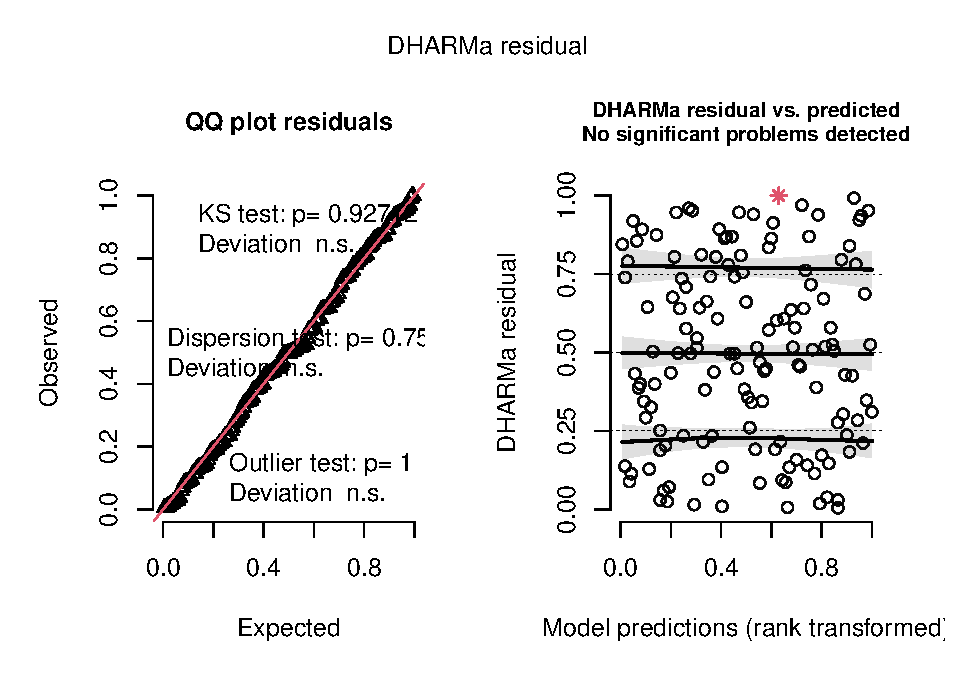
\includegraphics[keepaspectratio]{glmCH1_files/figure-latex/unnamed-chunk-10-1.pdf}}

\begin{Shaded}
\begin{Highlighting}[]
\DocumentationTok{\#\#residual plots show that there is no overdispersion and no excessive outliers. this shows that the negative binomial is a much better fit}
\end{Highlighting}
\end{Shaded}

Test zero-inflation

\begin{Shaded}
\begin{Highlighting}[]
\FunctionTok{testZeroInflation}\NormalTok{(residuals\_workers\_negbin)}
\end{Highlighting}
\end{Shaded}

\pandocbounded{
\includegraphics[keepaspectratio]{glmCH1_files/figure-latex/unnamed-chunk-11-1.pdf}}

\begin{verbatim}
## 
##  DHARMa zero-inflation test via comparison to expected zeros with
##  simulation under H0 = fitted model
## 
## data:  simulationOutput
## ratioObsSim = 1.0003, p-value = 1
## alternative hypothesis: two.sided
\end{verbatim}

\begin{Shaded}
\begin{Highlighting}[]
\DocumentationTok{\#\#p{-}value = 1. No evidence of zero{-}inflation. Do not fit zero{-}inflated model, leave as negative binomial.}
\end{Highlighting}
\end{Shaded}

Look at results of final model

\begin{Shaded}
\begin{Highlighting}[]
\FunctionTok{summary}\NormalTok{(worker\_lm\_negbin)}
\end{Highlighting}
\end{Shaded}

\begin{verbatim}
##  Family: nbinom1  ( log )
## Formula:          
## workers ~ nest_searching_queens_scaled + bombus_floral_abun_scaled +  
##     num_burrows_scaled + num_inactive_burrows_scaled + bee_season_type
## Data: field_data
## 
##       AIC       BIC    logLik -2*log(L)  df.resid 
##     163.0     183.6     -74.5     149.0       133 
## 
## 
## Dispersion parameter for nbinom1 family (): 1.94 
## 
## Conditional model:
##                              Estimate Std. Error z value Pr(>|z|)    
## (Intercept)                  -2.04281    0.61003  -3.349 0.000812 ***
## nest_searching_queens_scaled  0.05988    0.44176   0.136 0.892178    
## bombus_floral_abun_scaled     0.49887    0.27228   1.832 0.066917 .  
## num_burrows_scaled            0.09062    1.08744   0.083 0.933589    
## num_inactive_burrows_scaled   0.09220    0.81302   0.113 0.909706    
## bee_season_typeworker         0.92043    0.54647   1.684 0.092118 .  
## ---
## Signif. codes:  0 '***' 0.001 '**' 0.01 '*' 0.05 '.' 0.1 ' ' 1
\end{verbatim}

\section{GLM \#3: Number of burrows}\label{glm-3-number-of-burrows}

First, plot poisson

\begin{Shaded}
\begin{Highlighting}[]
\NormalTok{burrows\_lm\_pois }\OtherTok{\textless{}{-}} \FunctionTok{glmmTMB}\NormalTok{(num\_burrows }\SpecialCharTok{\textasciitilde{}}\NormalTok{ grass\_forb\_perc\_scaled }\SpecialCharTok{+} 
\NormalTok{                    julian.date\_scaled, }
                  \AttributeTok{family =}\NormalTok{ poisson, }\CommentTok{\#poisson}
                  \AttributeTok{data =}\NormalTok{ field\_data)}
\end{Highlighting}
\end{Shaded}

Diagnostics

\begin{Shaded}
\begin{Highlighting}[]
\CommentTok{\#simulate residuals}

\NormalTok{residuals\_burrows\_pois }\OtherTok{\textless{}{-}} \FunctionTok{simulateResiduals}\NormalTok{(}\AttributeTok{fittedModel =}\NormalTok{ burrows\_lm\_pois, }\AttributeTok{plot =} \ConstantTok{TRUE}\NormalTok{)}
\end{Highlighting}
\end{Shaded}

\begin{verbatim}
## Warning in newton(lsp = lsp, X = G$X, y = G$y, Eb = G$Eb, UrS = G$UrS, L = G$L,
## : Fitting terminated with step failure - check results carefully
\end{verbatim}

\pandocbounded{
\includegraphics[keepaspectratio]{glmCH1_files/figure-latex/unnamed-chunk-14-1.pdf}}

\begin{Shaded}
\begin{Highlighting}[]
\DocumentationTok{\#\#residual plots show that there is overdispersion and  excessive outliers. Plot negative binomial}
\end{Highlighting}
\end{Shaded}

Plot negative binomial to see if that fixes the overdispersion.

\begin{Shaded}
\begin{Highlighting}[]
\NormalTok{burrows\_lm\_negbin }\OtherTok{\textless{}{-}} \FunctionTok{glmmTMB}\NormalTok{(num\_burrows }\SpecialCharTok{\textasciitilde{}}\NormalTok{ grass\_forb\_perc\_scaled }\SpecialCharTok{+} 
\NormalTok{                    julian.date\_scaled, }
                  \AttributeTok{family =}\NormalTok{ nbinom1, }
                  \AttributeTok{data =}\NormalTok{ field\_data)}
\end{Highlighting}
\end{Shaded}

Diagnostics

\begin{Shaded}
\begin{Highlighting}[]
\CommentTok{\#simulate residuals}

\NormalTok{residuals\_burrows\_negbin }\OtherTok{\textless{}{-}} \FunctionTok{simulateResiduals}\NormalTok{(}\AttributeTok{fittedModel =}\NormalTok{ burrows\_lm\_negbin, }\AttributeTok{plot =} \ConstantTok{TRUE}\NormalTok{)}
\end{Highlighting}
\end{Shaded}

\pandocbounded{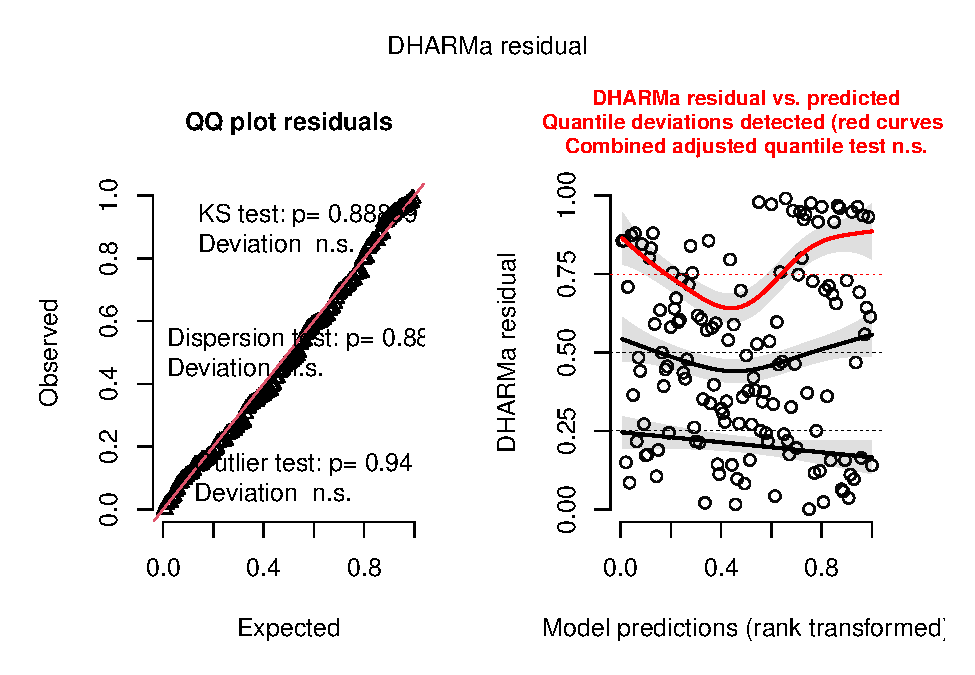
\includegraphics[keepaspectratio]{glmCH1_files/figure-latex/unnamed-chunk-16-1.pdf}}

\begin{Shaded}
\begin{Highlighting}[]
\DocumentationTok{\#\#residual plots show that there is no overdispersion or excessive outliers. Now check zero{-}inflation.}
\end{Highlighting}
\end{Shaded}

Test zero-inflation

\begin{Shaded}
\begin{Highlighting}[]
\FunctionTok{testZeroInflation}\NormalTok{(residuals\_burrows\_negbin)}
\end{Highlighting}
\end{Shaded}

\pandocbounded{
\includegraphics[keepaspectratio]{glmCH1_files/figure-latex/unnamed-chunk-17-1.pdf}}

\begin{verbatim}
## 
##  DHARMa zero-inflation test via comparison to expected zeros with
##  simulation under H0 = fitted model
## 
## data:  simulationOutput
## ratioObsSim = 0.81235, p-value = 0.256
## alternative hypothesis: two.sided
\end{verbatim}

\begin{Shaded}
\begin{Highlighting}[]
\DocumentationTok{\#\#p{-}value = 0.256. No strong evidence of zero{-}inflation. I\textquotesingle{}ll try the zero{-}inflated model to see if it helps. }
\end{Highlighting}
\end{Shaded}

Plot zero-inflated negative binomial and recheck diagnostics.

\begin{Shaded}
\begin{Highlighting}[]
\NormalTok{burrows\_lm\_zero\_negbin }\OtherTok{\textless{}{-}} \FunctionTok{glmmTMB}\NormalTok{(num\_burrows }\SpecialCharTok{\textasciitilde{}}\NormalTok{ grass\_forb\_perc\_scaled }\SpecialCharTok{+} 
\NormalTok{                    julian.date\_scaled, }
                    \AttributeTok{ziformula =} \SpecialCharTok{\textasciitilde{}}\DecValTok{1}\NormalTok{,  }\CommentTok{\# zero{-}inflation model}
                  \AttributeTok{family =}\NormalTok{ nbinom1, }
                  \AttributeTok{data =}\NormalTok{ field\_data)}
\end{Highlighting}
\end{Shaded}

Diagnostics

\begin{Shaded}
\begin{Highlighting}[]
\CommentTok{\#simulate residuals}

\NormalTok{residuals\_burrows\_zero\_negbin }\OtherTok{\textless{}{-}} \FunctionTok{simulateResiduals}\NormalTok{(}\AttributeTok{fittedModel =}\NormalTok{ burrows\_lm\_zero\_negbin, }\AttributeTok{plot =} \ConstantTok{TRUE}\NormalTok{)}
\end{Highlighting}
\end{Shaded}

\pandocbounded{
\includegraphics[keepaspectratio]{glmCH1_files/figure-latex/unnamed-chunk-19-1.pdf}}

\begin{Shaded}
\begin{Highlighting}[]
\DocumentationTok{\#\#residual plots does not look significantly better than the non{-}zero{-}inflated model.}
\end{Highlighting}
\end{Shaded}

Compare AIC values between the 2 models

\begin{Shaded}
\begin{Highlighting}[]
\FunctionTok{summary}\NormalTok{(burrows\_lm\_negbin)}
\end{Highlighting}
\end{Shaded}

\begin{verbatim}
##  Family: nbinom1  ( log )
## Formula:          num_burrows ~ grass_forb_perc_scaled + julian.date_scaled
## Data: field_data
## 
##       AIC       BIC    logLik -2*log(L)  df.resid 
##    1052.0    1063.7    -522.0    1044.0       136 
## 
## 
## Dispersion parameter for nbinom1 family (): 48.9 
## 
## Conditional model:
##                        Estimate Std. Error z value Pr(>|z|)    
## (Intercept)             3.11709    0.12941  24.086  < 2e-16 ***
## grass_forb_perc_scaled  0.43025    0.10936   3.934 8.35e-05 ***
## julian.date_scaled      0.08301    0.08634   0.961    0.336    
## ---
## Signif. codes:  0 '***' 0.001 '**' 0.01 '*' 0.05 '.' 0.1 ' ' 1
\end{verbatim}

\begin{Shaded}
\begin{Highlighting}[]
\FunctionTok{summary}\NormalTok{(burrows\_lm\_zero\_negbin)}
\end{Highlighting}
\end{Shaded}

\begin{verbatim}
##  Family: nbinom1  ( log )
## Formula:          num_burrows ~ grass_forb_perc_scaled + julian.date_scaled
## Zero inflation:               ~1
## Data: field_data
## 
##       AIC       BIC    logLik -2*log(L)  df.resid 
##    1054.0    1068.7    -522.0    1044.0       135 
## 
## 
## Dispersion parameter for nbinom1 family (): 48.9 
## 
## Conditional model:
##                        Estimate Std. Error z value Pr(>|z|)    
## (Intercept)             3.11709    0.12941  24.086  < 2e-16 ***
## grass_forb_perc_scaled  0.43026    0.10936   3.934 8.35e-05 ***
## julian.date_scaled      0.08301    0.08634   0.961    0.336    
## ---
## Signif. codes:  0 '***' 0.001 '**' 0.01 '*' 0.05 '.' 0.1 ' ' 1
## 
## Zero-inflation model:
##             Estimate Std. Error z value Pr(>|z|)
## (Intercept)   -20.08    4667.00  -0.004    0.997
\end{verbatim}

\begin{Shaded}
\begin{Highlighting}[]
\DocumentationTok{\#\#AIC and BIC values are slightly lover for negative binomial and there was no strong evidence for zero{-}inflation. Therefore, I think the negative binomal model is the best. }
\end{Highlighting}
\end{Shaded}

Results for the final model

\begin{Shaded}
\begin{Highlighting}[]
\FunctionTok{summary}\NormalTok{(burrows\_lm\_negbin)}
\end{Highlighting}
\end{Shaded}

\begin{verbatim}
##  Family: nbinom1  ( log )
## Formula:          num_burrows ~ grass_forb_perc_scaled + julian.date_scaled
## Data: field_data
## 
##       AIC       BIC    logLik -2*log(L)  df.resid 
##    1052.0    1063.7    -522.0    1044.0       136 
## 
## 
## Dispersion parameter for nbinom1 family (): 48.9 
## 
## Conditional model:
##                        Estimate Std. Error z value Pr(>|z|)    
## (Intercept)             3.11709    0.12941  24.086  < 2e-16 ***
## grass_forb_perc_scaled  0.43025    0.10936   3.934 8.35e-05 ***
## julian.date_scaled      0.08301    0.08634   0.961    0.336    
## ---
## Signif. codes:  0 '***' 0.001 '**' 0.01 '*' 0.05 '.' 0.1 ' ' 1
\end{verbatim}

\section{GLM \#4: Number of inactive rodent
burrows}\label{glm-4-number-of-inactive-rodent-burrows}

First, plot poisson

\begin{Shaded}
\begin{Highlighting}[]
\NormalTok{inactiveburrows\_lm\_pois }\OtherTok{\textless{}{-}} \FunctionTok{glmmTMB}\NormalTok{(num\_inactive\_burrows }\SpecialCharTok{\textasciitilde{}}\NormalTok{ grass\_forb\_perc\_scaled }\SpecialCharTok{+} 
\NormalTok{                    julian.date\_scaled, }
                  \AttributeTok{family =}\NormalTok{ poisson, }\CommentTok{\#poisson}
                  \AttributeTok{data =}\NormalTok{ field\_data)}
\end{Highlighting}
\end{Shaded}

Diagnostics

\begin{Shaded}
\begin{Highlighting}[]
\CommentTok{\#simulate residuals}

\NormalTok{residuals\_inactiveburrows\_pois }\OtherTok{\textless{}{-}} \FunctionTok{simulateResiduals}\NormalTok{(}\AttributeTok{fittedModel =}\NormalTok{ inactiveburrows\_lm\_pois, }\AttributeTok{plot =} \ConstantTok{TRUE}\NormalTok{)}
\end{Highlighting}
\end{Shaded}

\pandocbounded{
\includegraphics[keepaspectratio]{glmCH1_files/figure-latex/unnamed-chunk-23-1.pdf}}

\begin{Shaded}
\begin{Highlighting}[]
\DocumentationTok{\#\#residual plots show that there is overdispersion and  excessive outliers. Plot negative binomial}
\end{Highlighting}
\end{Shaded}

Plot negative binomial to see if that fixes the overdispersion.

\begin{Shaded}
\begin{Highlighting}[]
\NormalTok{inactiveburrows\_lm\_negbin }\OtherTok{\textless{}{-}} \FunctionTok{glmmTMB}\NormalTok{(num\_inactive\_burrows }\SpecialCharTok{\textasciitilde{}}\NormalTok{ grass\_forb\_perc\_scaled }\SpecialCharTok{+} 
\NormalTok{                    julian.date\_scaled, }
                  \AttributeTok{family =}\NormalTok{ nbinom1, }
                  \AttributeTok{data =}\NormalTok{ field\_data)}
\end{Highlighting}
\end{Shaded}

Diagnostics

\begin{Shaded}
\begin{Highlighting}[]
\CommentTok{\#simulate residuals}

\NormalTok{residuals\_inactiveburrows\_negbin }\OtherTok{\textless{}{-}} \FunctionTok{simulateResiduals}\NormalTok{(}\AttributeTok{fittedModel =}\NormalTok{ inactiveburrows\_lm\_negbin, }\AttributeTok{plot =} \ConstantTok{TRUE}\NormalTok{)}
\end{Highlighting}
\end{Shaded}

\pandocbounded{
\includegraphics[keepaspectratio]{glmCH1_files/figure-latex/unnamed-chunk-25-1.pdf}}

\begin{Shaded}
\begin{Highlighting}[]
\DocumentationTok{\#\#residual plots show that there is no overdispersion or excessive outliers. Now check zero{-}inflation.}
\end{Highlighting}
\end{Shaded}

Test zero-inflation

\begin{Shaded}
\begin{Highlighting}[]
\FunctionTok{testZeroInflation}\NormalTok{(residuals\_inactiveburrows\_negbin)}
\end{Highlighting}
\end{Shaded}

\pandocbounded{
\includegraphics[keepaspectratio]{glmCH1_files/figure-latex/unnamed-chunk-26-1.pdf}}

\begin{verbatim}
## 
##  DHARMa zero-inflation test via comparison to expected zeros with
##  simulation under H0 = fitted model
## 
## data:  simulationOutput
## ratioObsSim = 0.94158, p-value = 0.664
## alternative hypothesis: two.sided
\end{verbatim}

\begin{Shaded}
\begin{Highlighting}[]
\DocumentationTok{\#\#p{-}value = 0.664. No strong evidence of zero{-}inflation. I\textquotesingle{}ll try the zero{-}inflated model to see if it helps. }
\end{Highlighting}
\end{Shaded}

Plot zero-inflated negative binomial and recheck diagnostics.

\begin{Shaded}
\begin{Highlighting}[]
\NormalTok{inactiveburrows\_lm\_zero\_negbin }\OtherTok{\textless{}{-}} \FunctionTok{glmmTMB}\NormalTok{(num\_inactive\_burrows }\SpecialCharTok{\textasciitilde{}}\NormalTok{ grass\_forb\_perc\_scaled }\SpecialCharTok{+} 
\NormalTok{                    julian.date\_scaled, }
                    \AttributeTok{ziformula =} \SpecialCharTok{\textasciitilde{}}\DecValTok{1}\NormalTok{,  }\CommentTok{\# zero{-}inflation model}
                  \AttributeTok{family =}\NormalTok{ nbinom1, }
                  \AttributeTok{data =}\NormalTok{ field\_data)}
\end{Highlighting}
\end{Shaded}

Compare AIC values between the 2 models

\begin{Shaded}
\begin{Highlighting}[]
\FunctionTok{summary}\NormalTok{(inactiveburrows\_lm\_negbin)}
\end{Highlighting}
\end{Shaded}

\begin{verbatim}
##  Family: nbinom1  ( log )
## Formula:          
## num_inactive_burrows ~ grass_forb_perc_scaled + julian.date_scaled
## Data: field_data
## 
##       AIC       BIC    logLik -2*log(L)  df.resid 
##     817.7     829.4    -404.8     809.7       136 
## 
## 
## Dispersion parameter for nbinom1 family ():   22 
## 
## Conditional model:
##                        Estimate Std. Error z value Pr(>|z|)    
## (Intercept)             2.20210    0.13894  15.850  < 2e-16 ***
## grass_forb_perc_scaled  0.36568    0.12113   3.019  0.00254 ** 
## julian.date_scaled      0.08254    0.09534   0.866  0.38663    
## ---
## Signif. codes:  0 '***' 0.001 '**' 0.01 '*' 0.05 '.' 0.1 ' ' 1
\end{verbatim}

\begin{Shaded}
\begin{Highlighting}[]
\FunctionTok{summary}\NormalTok{(inactiveburrows\_lm\_zero\_negbin)}
\end{Highlighting}
\end{Shaded}

\begin{verbatim}
##  Family: nbinom1  ( log )
## Formula:          
## num_inactive_burrows ~ grass_forb_perc_scaled + julian.date_scaled
## Zero inflation:                        ~1
## Data: field_data
## 
##       AIC       BIC    logLik -2*log(L)  df.resid 
##     819.7     834.4    -404.8     809.7       135 
## 
## 
## Dispersion parameter for nbinom1 family ():   22 
## 
## Conditional model:
##                        Estimate Std. Error z value Pr(>|z|)    
## (Intercept)             2.20210    0.13894  15.849  < 2e-16 ***
## grass_forb_perc_scaled  0.36567    0.12113   3.019  0.00254 ** 
## julian.date_scaled      0.08253    0.09534   0.866  0.38667    
## ---
## Signif. codes:  0 '***' 0.001 '**' 0.01 '*' 0.05 '.' 0.1 ' ' 1
## 
## Zero-inflation model:
##             Estimate Std. Error z value Pr(>|z|)
## (Intercept)   -18.04    5337.31  -0.003    0.997
\end{verbatim}

\begin{Shaded}
\begin{Highlighting}[]
\DocumentationTok{\#\#AIC and BIC values are slightly lover for negative binomial and there was no strong evidence for zero{-}inflation. Therefore, I think the negative binomal model is the best. }
\end{Highlighting}
\end{Shaded}

Results for the final model

\begin{Shaded}
\begin{Highlighting}[]
\FunctionTok{summary}\NormalTok{(inactiveburrows\_lm\_negbin)}
\end{Highlighting}
\end{Shaded}

\begin{verbatim}
##  Family: nbinom1  ( log )
## Formula:          
## num_inactive_burrows ~ grass_forb_perc_scaled + julian.date_scaled
## Data: field_data
## 
##       AIC       BIC    logLik -2*log(L)  df.resid 
##     817.7     829.4    -404.8     809.7       136 
## 
## 
## Dispersion parameter for nbinom1 family ():   22 
## 
## Conditional model:
##                        Estimate Std. Error z value Pr(>|z|)    
## (Intercept)             2.20210    0.13894  15.850  < 2e-16 ***
## grass_forb_perc_scaled  0.36568    0.12113   3.019  0.00254 ** 
## julian.date_scaled      0.08254    0.09534   0.866  0.38663    
## ---
## Signif. codes:  0 '***' 0.001 '**' 0.01 '*' 0.05 '.' 0.1 ' ' 1
\end{verbatim}

\section{GLM \#5: Floral abundance}\label{glm-5-floral-abundance}

Plot gamma regression since distribution of floral abundance across
sites is positive and right-skewed.

\begin{Shaded}
\begin{Highlighting}[]
\NormalTok{floral\_lm\_tweedie }\OtherTok{\textless{}{-}} \FunctionTok{glmmTMB}\NormalTok{(bombus\_floral\_abun }\SpecialCharTok{\textasciitilde{}}\NormalTok{ grass\_forb\_perc\_scaled }\SpecialCharTok{+} 
\NormalTok{                    julian.date\_scaled, }
                  \AttributeTok{family =} \FunctionTok{tweedie}\NormalTok{(}\AttributeTok{link =} \StringTok{"log"}\NormalTok{), }\DocumentationTok{\#\#use tweedie family instead of Gamma since it can handle zeros and positive continuous data}
                  \AttributeTok{data =}\NormalTok{ field\_data)}
\end{Highlighting}
\end{Shaded}

Diagnostics

\begin{Shaded}
\begin{Highlighting}[]
\CommentTok{\#simulate residuals}

\NormalTok{residuals\_floral\_tweedie }\OtherTok{\textless{}{-}} \FunctionTok{simulateResiduals}\NormalTok{(}\AttributeTok{fittedModel =}\NormalTok{ floral\_lm\_tweedie, }\AttributeTok{plot =} \ConstantTok{TRUE}\NormalTok{)}
\end{Highlighting}
\end{Shaded}

\pandocbounded{
\includegraphics[keepaspectratio]{glmCH1_files/figure-latex/unnamed-chunk-31-1.pdf}}

\begin{Shaded}
\begin{Highlighting}[]
\DocumentationTok{\#\#residual plots show that there is overdispersion and  excessive outliers.}
\end{Highlighting}
\end{Shaded}

Try plotting the log(floral abundance) as a linear regression

\begin{Shaded}
\begin{Highlighting}[]
\NormalTok{field\_data}\SpecialCharTok{$}\NormalTok{log\_bombus\_floral\_abun }\OtherTok{\textless{}{-}} \FunctionTok{log}\NormalTok{(field\_data}\SpecialCharTok{$}\NormalTok{bombus\_floral\_abun }\SpecialCharTok{+} \FloatTok{1e{-}4}\NormalTok{)}

\NormalTok{floral\_lm\_log }\OtherTok{\textless{}{-}} \FunctionTok{lm}\NormalTok{(log\_bombus\_floral\_abun }\SpecialCharTok{\textasciitilde{}}\NormalTok{ grass\_forb\_perc\_scaled }\SpecialCharTok{+}\NormalTok{ julian.date\_scaled, }\AttributeTok{data =}\NormalTok{ field\_data)}
\end{Highlighting}
\end{Shaded}

Diagnostics

\begin{Shaded}
\begin{Highlighting}[]
\NormalTok{residuals\_floral\_log }\OtherTok{\textless{}{-}} \FunctionTok{simulateResiduals}\NormalTok{(}\AttributeTok{fittedModel =}\NormalTok{ floral\_lm\_log, }\AttributeTok{plot =} \ConstantTok{TRUE}\NormalTok{)}
\end{Highlighting}
\end{Shaded}

\pandocbounded{
\includegraphics[keepaspectratio]{glmCH1_files/figure-latex/unnamed-chunk-33-1.pdf}}

\begin{Shaded}
\begin{Highlighting}[]
\DocumentationTok{\#\#fixed overdispersion and outliers. KS test suggests non{-}normality but I will check this in the Q{-}Q plot}

\FunctionTok{library}\NormalTok{(car)}
\end{Highlighting}
\end{Shaded}

\begin{verbatim}
## Loading required package: carData
\end{verbatim}

\begin{verbatim}
## 
## Attaching package: 'car'
\end{verbatim}

\begin{verbatim}
## The following object is masked from 'package:dplyr':
## 
##     recode
\end{verbatim}

\begin{verbatim}
## The following object is masked from 'package:purrr':
## 
##     some
\end{verbatim}

\begin{Shaded}
\begin{Highlighting}[]
\FunctionTok{qqPlot}\NormalTok{(floral\_lm\_log, }\AttributeTok{main =} \StringTok{"Q{-}Q Plot"}\NormalTok{)}
\end{Highlighting}
\end{Shaded}

\pandocbounded{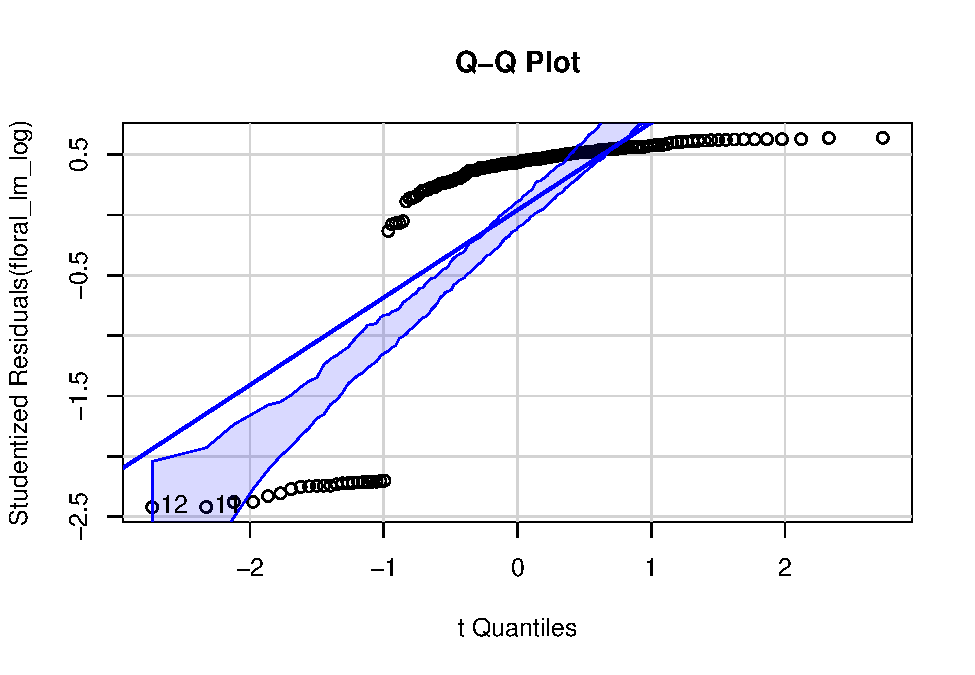
\includegraphics[keepaspectratio]{glmCH1_files/figure-latex/unnamed-chunk-33-2.pdf}}

\begin{verbatim}
## [1] 11 12
\end{verbatim}

\begin{Shaded}
\begin{Highlighting}[]
\DocumentationTok{\#\#Q{-}Q plot shows that residuals are still not normal. Need to try a different model.}
\end{Highlighting}
\end{Shaded}

Try running Tweedie model again but adjusting for overdispersion by
adding a random effect for data structure

\begin{Shaded}
\begin{Highlighting}[]
\NormalTok{floral\_glmm\_tweedie }\OtherTok{\textless{}{-}} \FunctionTok{glmmTMB}\NormalTok{(bombus\_floral\_abun }\SpecialCharTok{\textasciitilde{}}\NormalTok{ grass\_forb\_perc\_scaled }\SpecialCharTok{+} 
\NormalTok{                    julian.date\_scaled }\SpecialCharTok{+}\NormalTok{ (}\DecValTok{1}\SpecialCharTok{|}\NormalTok{area}\SpecialCharTok{/}\NormalTok{site\_id}\SpecialCharTok{/}\NormalTok{plot\_id), }
                  \AttributeTok{family =} \FunctionTok{tweedie}\NormalTok{(}\AttributeTok{link =} \StringTok{"log"}\NormalTok{), }
                  \AttributeTok{data =}\NormalTok{ field\_data)}
\end{Highlighting}
\end{Shaded}

Diagnostics

\begin{Shaded}
\begin{Highlighting}[]
\CommentTok{\#simulate residuals}

\NormalTok{residuals\_floral\_tweedie\_mixed }\OtherTok{\textless{}{-}} \FunctionTok{simulateResiduals}\NormalTok{(}\AttributeTok{fittedModel =}\NormalTok{ floral\_glmm\_tweedie, }\AttributeTok{plot =} \ConstantTok{TRUE}\NormalTok{)}
\end{Highlighting}
\end{Shaded}

\begin{verbatim}
## Warning in newton(lsp = lsp, X = G$X, y = G$y, Eb = G$Eb, UrS = G$UrS, L = G$L,
## : Fitting terminated with step failure - check results carefully
\end{verbatim}

\pandocbounded{
\includegraphics[keepaspectratio]{glmCH1_files/figure-latex/unnamed-chunk-35-1.pdf}}

\begin{Shaded}
\begin{Highlighting}[]
\DocumentationTok{\#\#residual plots show that there is still overdispersion. try different random effect.}
\end{Highlighting}
\end{Shaded}

Try simpler random effect structure (ignore site)

\begin{Shaded}
\begin{Highlighting}[]
\NormalTok{floral\_glmm\_tweedie2 }\OtherTok{\textless{}{-}} \FunctionTok{glmmTMB}\NormalTok{(bombus\_floral\_abun }\SpecialCharTok{\textasciitilde{}}\NormalTok{ grass\_forb\_perc\_scaled }\SpecialCharTok{+} 
\NormalTok{                    julian.date\_scaled }\SpecialCharTok{+}\NormalTok{ (}\DecValTok{1}\SpecialCharTok{|}\NormalTok{area}\SpecialCharTok{/}\NormalTok{plot\_id), }
                  \AttributeTok{family =} \FunctionTok{tweedie}\NormalTok{(}\AttributeTok{link =} \StringTok{"log"}\NormalTok{), }
                  \AttributeTok{data =}\NormalTok{ field\_data)}
\end{Highlighting}
\end{Shaded}

Diagnostics --check for overdispersion

\begin{Shaded}
\begin{Highlighting}[]
\NormalTok{sim\_res }\OtherTok{\textless{}{-}} \FunctionTok{simulateResiduals}\NormalTok{(floral\_glmm\_tweedie2)}
\FunctionTok{plot}\NormalTok{(sim\_res)}
\end{Highlighting}
\end{Shaded}

\pandocbounded{
\includegraphics[keepaspectratio]{glmCH1_files/figure-latex/unnamed-chunk-37-1.pdf}}

\begin{Shaded}
\begin{Highlighting}[]
\FunctionTok{testDispersion}\NormalTok{(sim\_res)}
\end{Highlighting}
\end{Shaded}

\pandocbounded{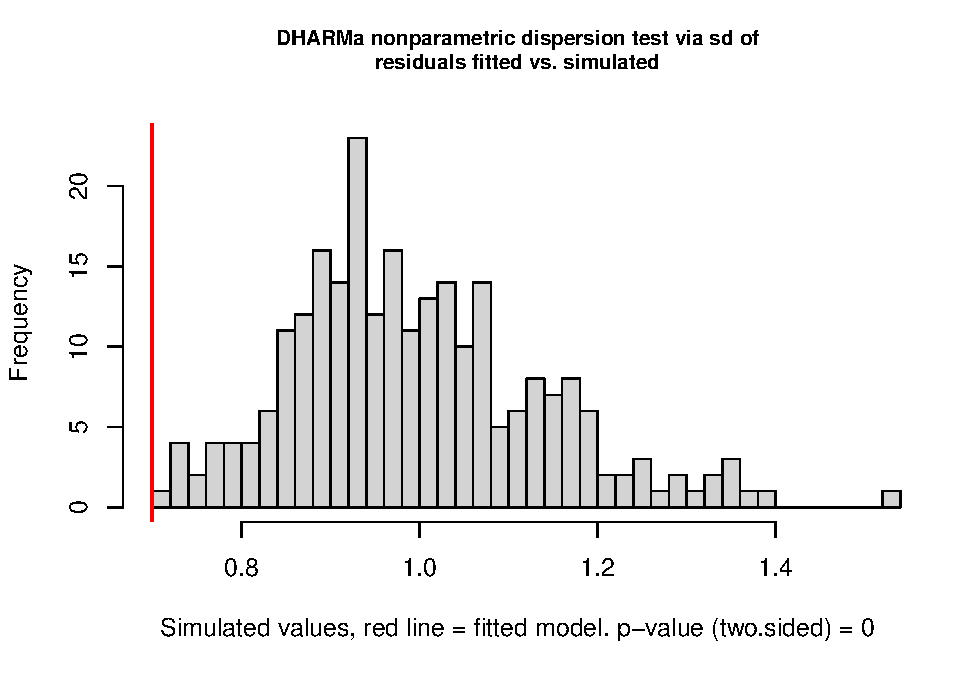
\includegraphics[keepaspectratio]{glmCH1_files/figure-latex/unnamed-chunk-37-2.pdf}}

\begin{verbatim}
## 
##  DHARMa nonparametric dispersion test via sd of residuals fitted vs.
##  simulated
## 
## data:  simulationOutput
## dispersion = 0.70199, p-value < 2.2e-16
## alternative hypothesis: two.sided
\end{verbatim}

\begin{Shaded}
\begin{Highlighting}[]
\DocumentationTok{\#\#still overdispersion. Keep original random effect structure for now but try modelling zero{-}inflation in model}
\end{Highlighting}
\end{Shaded}

Zero-inflated model

\begin{Shaded}
\begin{Highlighting}[]
\NormalTok{floral\_glmm\_tweediezero }\OtherTok{\textless{}{-}} \FunctionTok{glmmTMB}\NormalTok{(bombus\_floral\_abun }\SpecialCharTok{\textasciitilde{}}\NormalTok{ grass\_forb\_perc\_scaled }\SpecialCharTok{+} 
\NormalTok{                    julian.date\_scaled }\SpecialCharTok{+}\NormalTok{ (}\DecValTok{1}\SpecialCharTok{|}\NormalTok{area}\SpecialCharTok{/}\NormalTok{site\_id}\SpecialCharTok{/}\NormalTok{plot\_id), }
                    \AttributeTok{ziformula =} \SpecialCharTok{\textasciitilde{}}\DecValTok{1}\NormalTok{, }\CommentTok{\#zero{-}inflated model}
                  \AttributeTok{family =} \FunctionTok{tweedie}\NormalTok{(}\AttributeTok{link =} \StringTok{"log"}\NormalTok{), }
                  \AttributeTok{data =}\NormalTok{ field\_data)}
\end{Highlighting}
\end{Shaded}

Diagnostics --check for overdispersion

\begin{Shaded}
\begin{Highlighting}[]
\NormalTok{sim\_res }\OtherTok{\textless{}{-}} \FunctionTok{simulateResiduals}\NormalTok{(floral\_glmm\_tweediezero)}
\FunctionTok{plot}\NormalTok{(sim\_res)}
\end{Highlighting}
\end{Shaded}

\pandocbounded{
\includegraphics[keepaspectratio]{glmCH1_files/figure-latex/unnamed-chunk-39-1.pdf}}

\begin{Shaded}
\begin{Highlighting}[]
\FunctionTok{testDispersion}\NormalTok{(sim\_res)}
\end{Highlighting}
\end{Shaded}

\pandocbounded{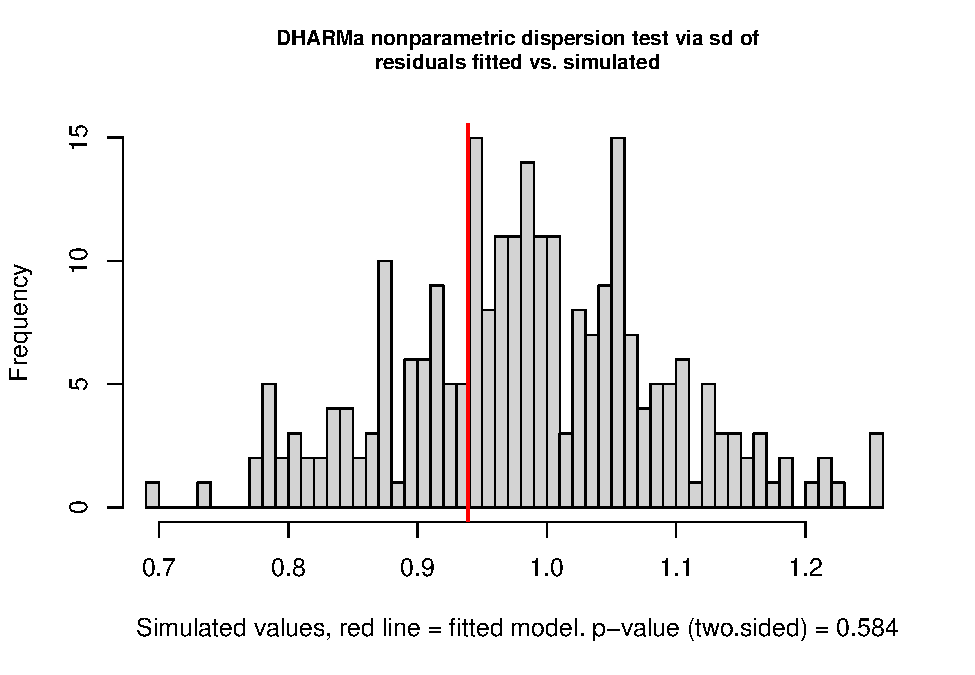
\includegraphics[keepaspectratio]{glmCH1_files/figure-latex/unnamed-chunk-39-2.pdf}}

\begin{verbatim}
## 
##  DHARMa nonparametric dispersion test via sd of residuals fitted vs.
##  simulated
## 
## data:  simulationOutput
## dispersion = 0.95183, p-value = 0.584
## alternative hypothesis: two.sided
\end{verbatim}

\begin{Shaded}
\begin{Highlighting}[]
\DocumentationTok{\#\#no more overdispersion!}
\end{Highlighting}
\end{Shaded}

Check other random effect structures to determine which is best

\begin{Shaded}
\begin{Highlighting}[]
\CommentTok{\#plot nested in area (drop site)}

\NormalTok{floral\_glmm\_tweediezero\_plot }\OtherTok{\textless{}{-}} \FunctionTok{glmmTMB}\NormalTok{(bombus\_floral\_abun }\SpecialCharTok{\textasciitilde{}}\NormalTok{ grass\_forb\_perc\_scaled }\SpecialCharTok{+} 
\NormalTok{                    julian.date\_scaled }\SpecialCharTok{+}\NormalTok{ (}\DecValTok{1}\SpecialCharTok{|}\NormalTok{area}\SpecialCharTok{/}\NormalTok{plot\_id), }
                    \AttributeTok{ziformula =} \SpecialCharTok{\textasciitilde{}}\DecValTok{1}\NormalTok{, }\CommentTok{\#zero{-}inflated model}
                  \AttributeTok{family =} \FunctionTok{tweedie}\NormalTok{(}\AttributeTok{link =} \StringTok{"log"}\NormalTok{), }
                  \AttributeTok{data =}\NormalTok{ field\_data)}

\CommentTok{\#site nested in area (drop plot)}

\NormalTok{floral\_glmm\_tweediezero\_site }\OtherTok{\textless{}{-}} \FunctionTok{glmmTMB}\NormalTok{(bombus\_floral\_abun }\SpecialCharTok{\textasciitilde{}}\NormalTok{ grass\_forb\_perc\_scaled }\SpecialCharTok{+} 
\NormalTok{                    julian.date\_scaled }\SpecialCharTok{+}\NormalTok{ (}\DecValTok{1}\SpecialCharTok{|}\NormalTok{area}\SpecialCharTok{/}\NormalTok{site\_id), }
                    \AttributeTok{ziformula =} \SpecialCharTok{\textasciitilde{}}\DecValTok{1}\NormalTok{, }\CommentTok{\#zero{-}inflated model}
                  \AttributeTok{family =} \FunctionTok{tweedie}\NormalTok{(}\AttributeTok{link =} \StringTok{"log"}\NormalTok{), }
                  \AttributeTok{data =}\NormalTok{ field\_data)}

\CommentTok{\#plot only}

\NormalTok{floral\_glmm\_tweediezero\_plotonly }\OtherTok{\textless{}{-}} \FunctionTok{glmmTMB}\NormalTok{(bombus\_floral\_abun }\SpecialCharTok{\textasciitilde{}}\NormalTok{ grass\_forb\_perc\_scaled }\SpecialCharTok{+} 
\NormalTok{                    julian.date\_scaled }\SpecialCharTok{+}\NormalTok{ (}\DecValTok{1}\SpecialCharTok{|}\NormalTok{plot\_id), }
                    \AttributeTok{ziformula =} \SpecialCharTok{\textasciitilde{}}\DecValTok{1}\NormalTok{, }\CommentTok{\#zero{-}inflated model}
                  \AttributeTok{family =} \FunctionTok{tweedie}\NormalTok{(}\AttributeTok{link =} \StringTok{"log"}\NormalTok{), }
                  \AttributeTok{data =}\NormalTok{ field\_data)}

\CommentTok{\#site only}

\NormalTok{floral\_glmm\_tweediezero\_siteonly }\OtherTok{\textless{}{-}} \FunctionTok{glmmTMB}\NormalTok{(bombus\_floral\_abun }\SpecialCharTok{\textasciitilde{}}\NormalTok{ grass\_forb\_perc\_scaled }\SpecialCharTok{+} 
\NormalTok{                    julian.date\_scaled }\SpecialCharTok{+}\NormalTok{ (}\DecValTok{1}\SpecialCharTok{|}\NormalTok{site\_id), }
                    \AttributeTok{ziformula =} \SpecialCharTok{\textasciitilde{}}\DecValTok{1}\NormalTok{, }\CommentTok{\#zero{-}inflated model}
                  \AttributeTok{family =} \FunctionTok{tweedie}\NormalTok{(}\AttributeTok{link =} \StringTok{"log"}\NormalTok{), }
                  \AttributeTok{data =}\NormalTok{ field\_data)}

\CommentTok{\#area only}

\NormalTok{floral\_glmm\_tweediezero\_areaonly }\OtherTok{\textless{}{-}} \FunctionTok{glmmTMB}\NormalTok{(bombus\_floral\_abun }\SpecialCharTok{\textasciitilde{}}\NormalTok{ grass\_forb\_perc\_scaled }\SpecialCharTok{+} 
\NormalTok{                    julian.date\_scaled }\SpecialCharTok{+}\NormalTok{ (}\DecValTok{1}\SpecialCharTok{|}\NormalTok{area), }
                    \AttributeTok{ziformula =} \SpecialCharTok{\textasciitilde{}}\DecValTok{1}\NormalTok{, }\CommentTok{\#zero{-}inflated model}
                  \AttributeTok{family =} \FunctionTok{tweedie}\NormalTok{(}\AttributeTok{link =} \StringTok{"log"}\NormalTok{), }
                  \AttributeTok{data =}\NormalTok{ field\_data)}

\CommentTok{\#check AIC}
\FunctionTok{AIC}\NormalTok{(}
\NormalTok{  floral\_glmm\_tweediezero, }
\NormalTok{  floral\_glmm\_tweediezero\_plot,}
\NormalTok{  floral\_glmm\_tweediezero\_site,}
\NormalTok{  floral\_glmm\_tweediezero\_plotonly, }
\NormalTok{  floral\_glmm\_tweediezero\_siteonly, }
\NormalTok{  floral\_glmm\_tweediezero\_areaonly}
\NormalTok{)}
\end{Highlighting}
\end{Shaded}

\begin{verbatim}
##                                  df      AIC
## floral_glmm_tweediezero           9 516.2534
## floral_glmm_tweediezero_plot      8 514.2534
## floral_glmm_tweediezero_site      8 513.1628
## floral_glmm_tweediezero_plotonly  7 487.1094
## floral_glmm_tweediezero_siteonly  7 512.3448
## floral_glmm_tweediezero_areaonly  7 512.2534
\end{verbatim}

\begin{Shaded}
\begin{Highlighting}[]
\DocumentationTok{\#\#plot only model has lowest AIC{-}{-}\textgreater{} go with that one!}
\end{Highlighting}
\end{Shaded}

Check overdispersion in plot only model

\begin{Shaded}
\begin{Highlighting}[]
\NormalTok{sim\_res }\OtherTok{\textless{}{-}} \FunctionTok{simulateResiduals}\NormalTok{(floral\_glmm\_tweediezero\_plotonly)}
\FunctionTok{plot}\NormalTok{(sim\_res)}
\end{Highlighting}
\end{Shaded}

\pandocbounded{
\includegraphics[keepaspectratio]{glmCH1_files/figure-latex/unnamed-chunk-41-1.pdf}}

\begin{Shaded}
\begin{Highlighting}[]
\FunctionTok{testDispersion}\NormalTok{(sim\_res)}
\end{Highlighting}
\end{Shaded}

\pandocbounded{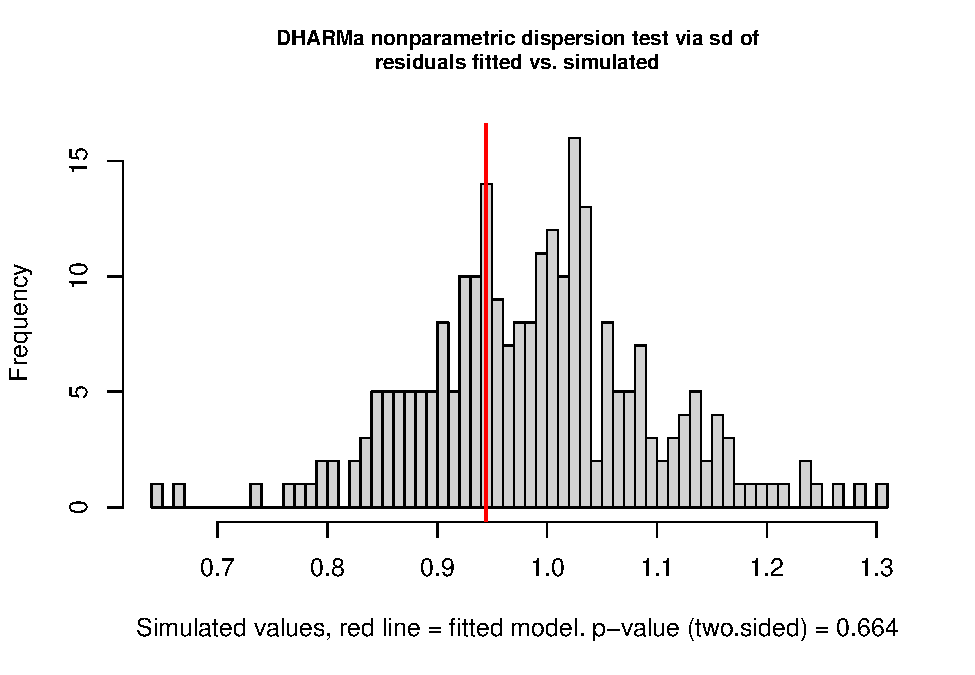
\includegraphics[keepaspectratio]{glmCH1_files/figure-latex/unnamed-chunk-41-2.pdf}}

\begin{verbatim}
## 
##  DHARMa nonparametric dispersion test via sd of residuals fitted vs.
##  simulated
## 
## data:  simulationOutput
## dispersion = 0.95435, p-value = 0.664
## alternative hypothesis: two.sided
\end{verbatim}

\begin{Shaded}
\begin{Highlighting}[]
\DocumentationTok{\#\#still no overdispersion}
\end{Highlighting}
\end{Shaded}

Look at summary for final model

\begin{Shaded}
\begin{Highlighting}[]
\FunctionTok{summary}\NormalTok{(floral\_glmm\_tweediezero\_plotonly)}
\end{Highlighting}
\end{Shaded}

\begin{verbatim}
##  Family: tweedie  ( log )
## Formula:          
## bombus_floral_abun ~ grass_forb_perc_scaled + julian.date_scaled +  
##     (1 | plot_id)
## Zero inflation:                      ~1
## Data: field_data
## 
##       AIC       BIC    logLik -2*log(L)  df.resid 
##     487.1     507.7    -236.6     473.1       133 
## 
## Random effects:
## 
## Conditional model:
##  Groups  Name        Variance  Std.Dev. 
##  plot_id (Intercept) 1.087e-10 1.043e-05
## Number of obs: 140, groups:  plot_id, 2
## 
## Dispersion parameter for tweedie family ():  0.5 
## 
## Conditional model:
##                         Estimate Std. Error z value Pr(>|z|)    
## (Intercept)             1.068626   0.040817  26.181   <2e-16 ***
## grass_forb_perc_scaled -0.009948   0.047577  -0.209    0.834    
## julian.date_scaled     -0.067595   0.041604  -1.625    0.104    
## ---
## Signif. codes:  0 '***' 0.001 '**' 0.01 '*' 0.05 '.' 0.1 ' ' 1
## 
## Zero-inflation model:
##             Estimate Std. Error z value Pr(>|z|)    
## (Intercept)  -1.6457     0.2318    -7.1 1.25e-12 ***
## ---
## Signif. codes:  0 '***' 0.001 '**' 0.01 '*' 0.05 '.' 0.1 ' ' 1
\end{verbatim}

\end{document}
